\documentclass[a4paper, 12pt]{article}
\usepackage{graphicx}
\usepackage[T2A]{fontenc}
\usepackage[utf8]{inputenc}
\usepackage[english,russian]{babel}
\usepackage{listings}
\usepackage{multirow}
\usepackage{pgfplots}
\usepackage{pgfplotstable}
\usepackage[normalem]{ulem}
\usepackage{geometry}
\usepackage{amsmath}
\usepackage{titlesec}

\usepgfplotslibrary{units}
\pgfplotsset{compat=1.16}
\geometry{left=25mm, right=10mm, top=20mm, bottom=20mm}

\renewcommand{\thepart}{\arabic{part}}
\renewcommand{\thesection}{\thepart.\arabic{section}}


\begin{document}
    \thispagestyle{empty}

\begin{center}
    Санкт-Петербургский политехнический университет Петра Великого\\
    Институт Компьютерных Наук и Технологий\\
    \bfseries{Кафедра «Высшая школа программной инженерии»}
\end{center}

\vspace{20ex}

\begin{center}
{
\LARGE \textbf{Курсовой проект} \\[3ex]
по дисциплине: «Микропроцессорные системы»
}
\end{center}

\vspace{40ex}

\noindent Выполнил\\
студент гр.33534/21\hfill
\begin{minipage}{0.7\textwidth}
    \hfill \uline{\hspace{3cm}} \hspace{1.1cm} С.А. Фомин
\end{minipage}

\vspace{3ex}

\noindent Проверил\\
преподаватель\hfill
\begin{minipage}{0.7\textwidth}
    \hfill \uline{\hspace{3cm}} \hspace{0.5cm} С.К. Круглов
\end{minipage}

\vspace{3ex}

\vfill

\begin{center}
    Санкт-Петербург\\
    2018
\end{center}



    \newpage

    \section*{Формулировка задачи}
        Разработать клиент-серверное приложение для вывода на внешний жидкокристаллический
        дисплей (с помощью Raspberry Pi) количества сокращенных ссылок из базы данных сервиса short.taxnuke.ru в режиме реального времени.

    \section*{Ход работы}
        В качестве программной среды было принятно решение использовать Node.js - кроссплатформенное решение,
        использующее в качестве JavaScript-движка V8, написанный на C. Для Node.js имеется множество готовых библиотек
        на JavaScript с биндингами к нативным модулям на C++ и C и с многопоточностью.
        Выбор обусловлен тем, что изначально сервис short.taxnuke.ru тоже написан Node.js и использоание
        одной программной среды и языка позволяет минимизировать количество зависимостей и упростить интерфейс между компонентами.
        Также Node.js позволяет порождать дочерние процессы и передавать в них аргументы командной
        строки, управляющие последовательности и использовать потоки ввода/вывода.

        \begin{figure}
            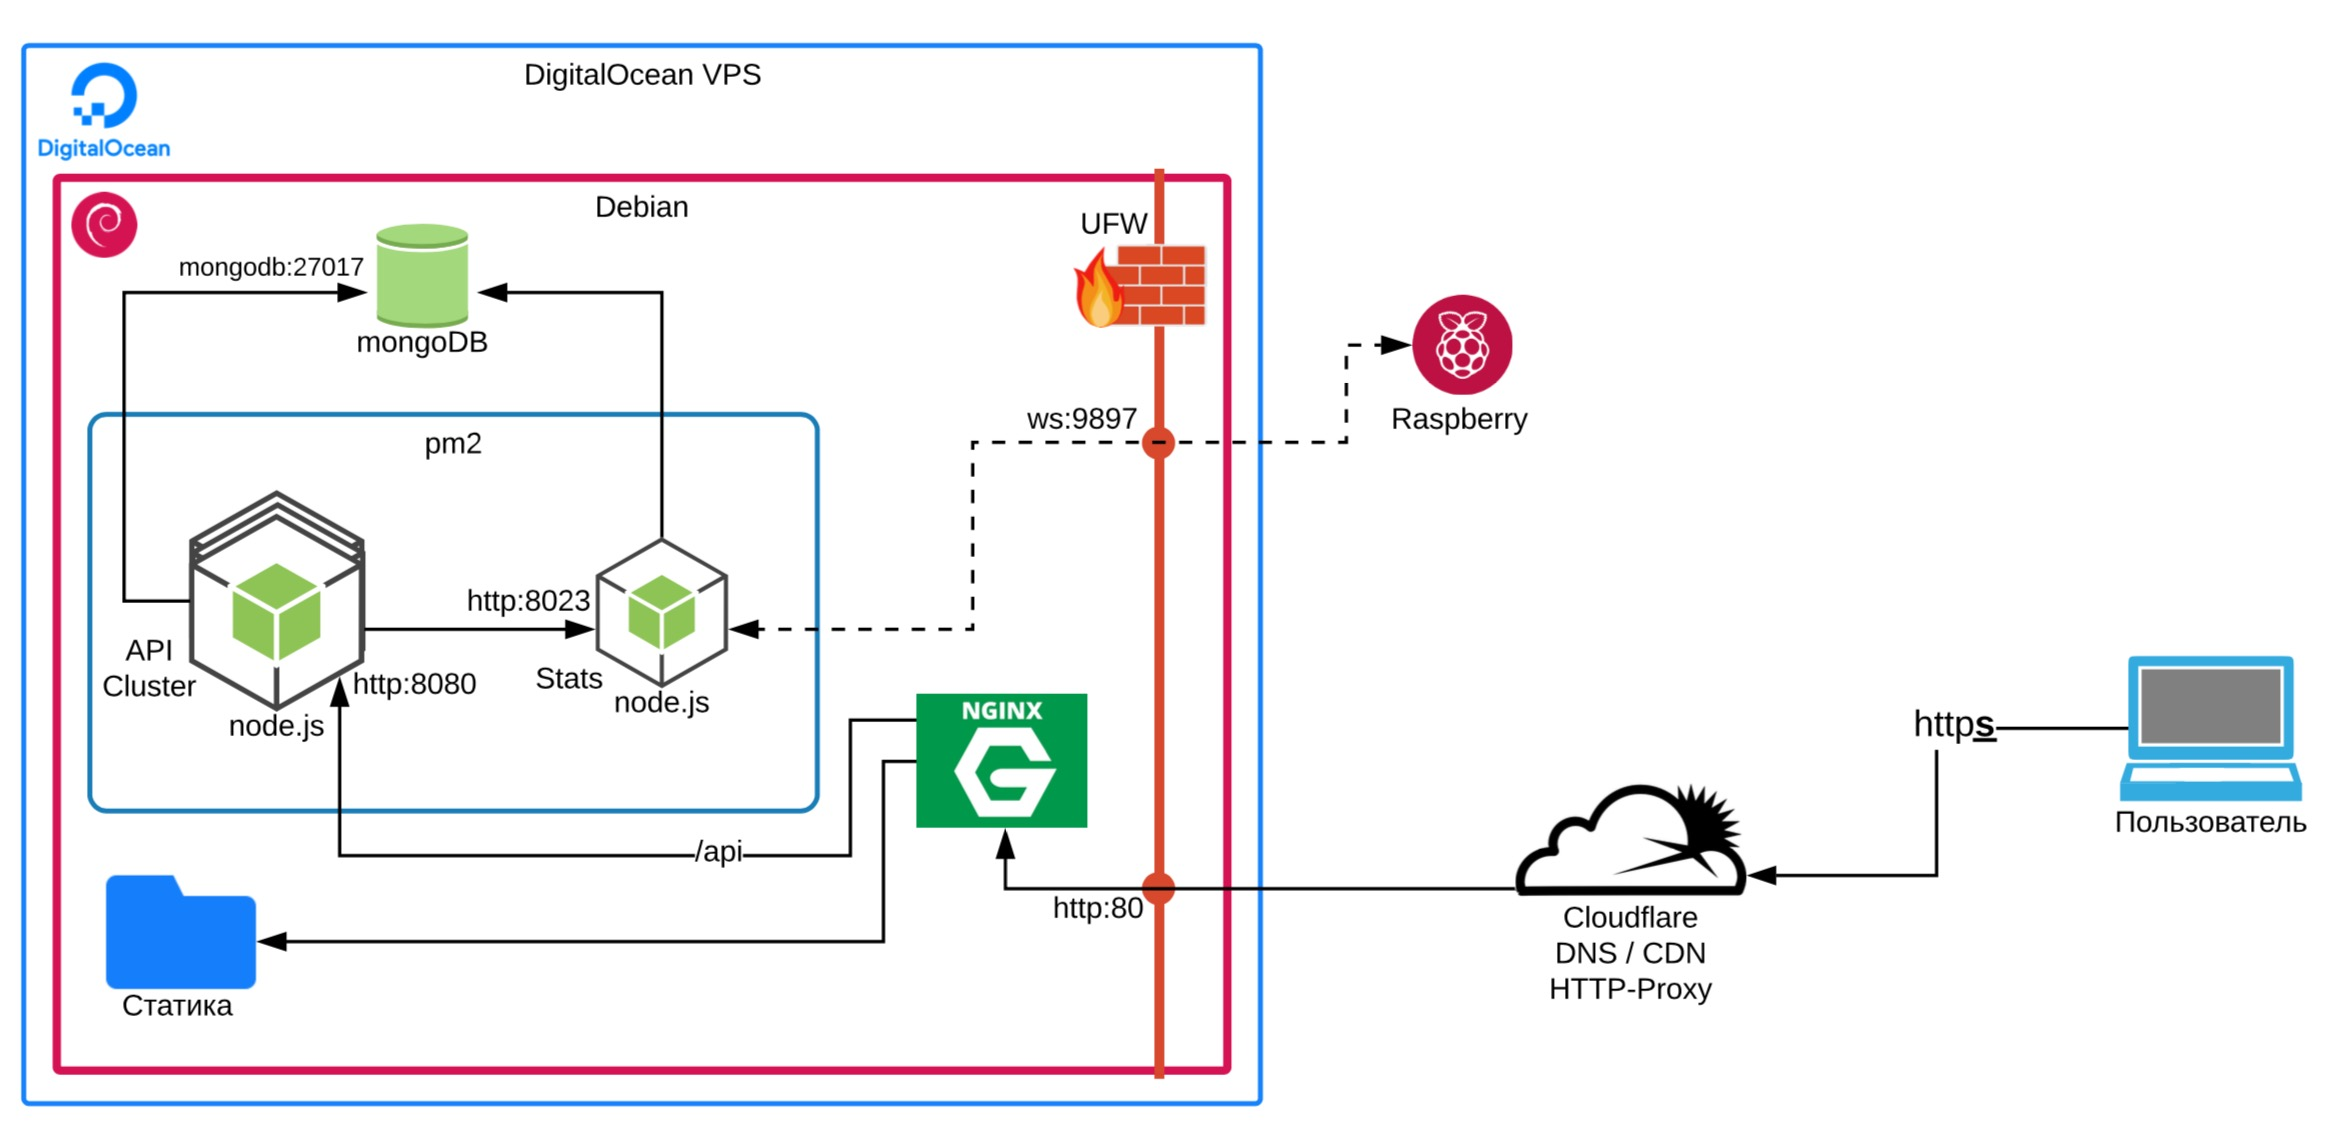
\includegraphics[width=\linewidth]{img/arch.jpg}
            \caption{Схема архитектуры крупным планом.}
            \label{fig:bigarch}
        \end{figure}

        На рисунке~\ref{fig:bigarch} изображена схема сервиса short.taxnuke.ru в целом, а также интегрированного в него
        клиент-серверного приложения для отображения статистики.

    \section*{Результат работы}
    \section*{Вывод}


\end{document}
